\section{Subject Behavior Diagram Interpretation}

%appendix in smaller font size
\footnotesize

\begin{figure}[ph]
	\centering
	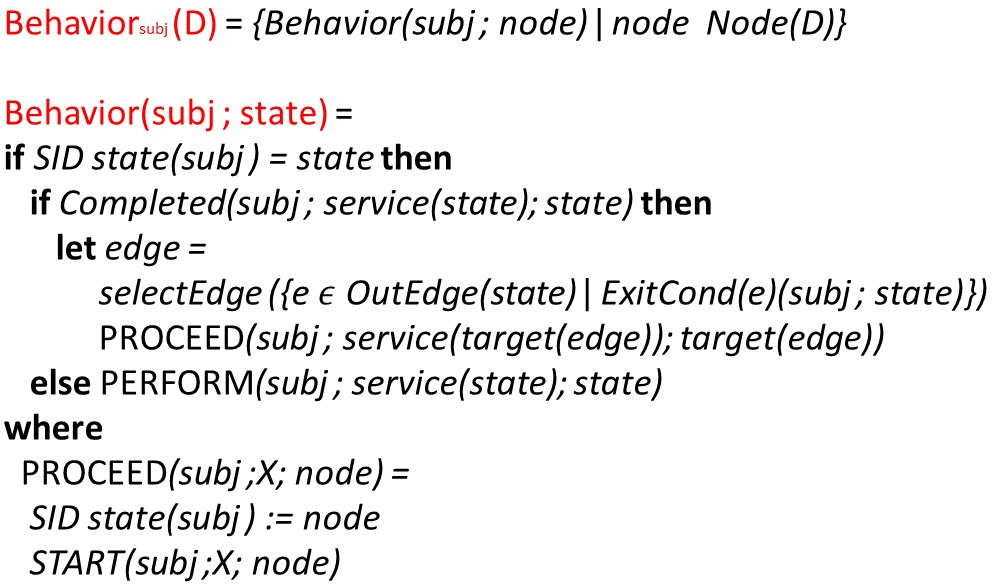
\includegraphics[width=0.7\linewidth]{20181026-Ontologie-Bilder/Grafiken-Ontologie/SUbjectExecution/ASM-Behavior}
\caption[Top Level of Interpreter Model]{Top Level of Interpreter Model}
	\label{fig:asm-behavior}
\end{figure}

\newpage
\section{Alternative Send/Receive Round Interpretation}

\begin{figure}[ph]
	\centering
	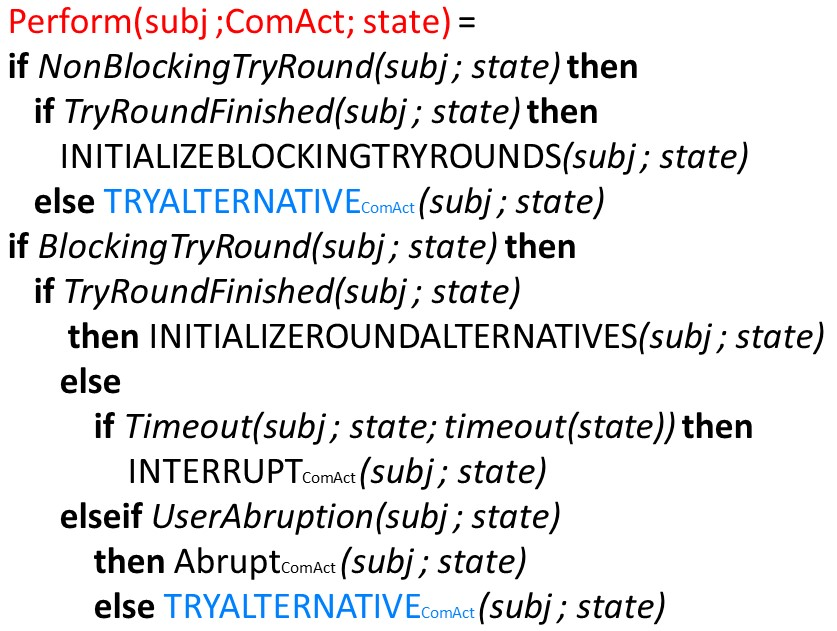
\includegraphics[width=0.8\linewidth]{20181026-Ontologie-Bilder/Grafiken-Ontologie/SUbjectExecution/ASM-perform}
	\caption[Alternative Send/Receive Round Interpretation]{Alternative Send/Receive Round Interpretation}
	\label{fig:asm-perform}
\end{figure}

\begin{figure}[ph]
	\centering
	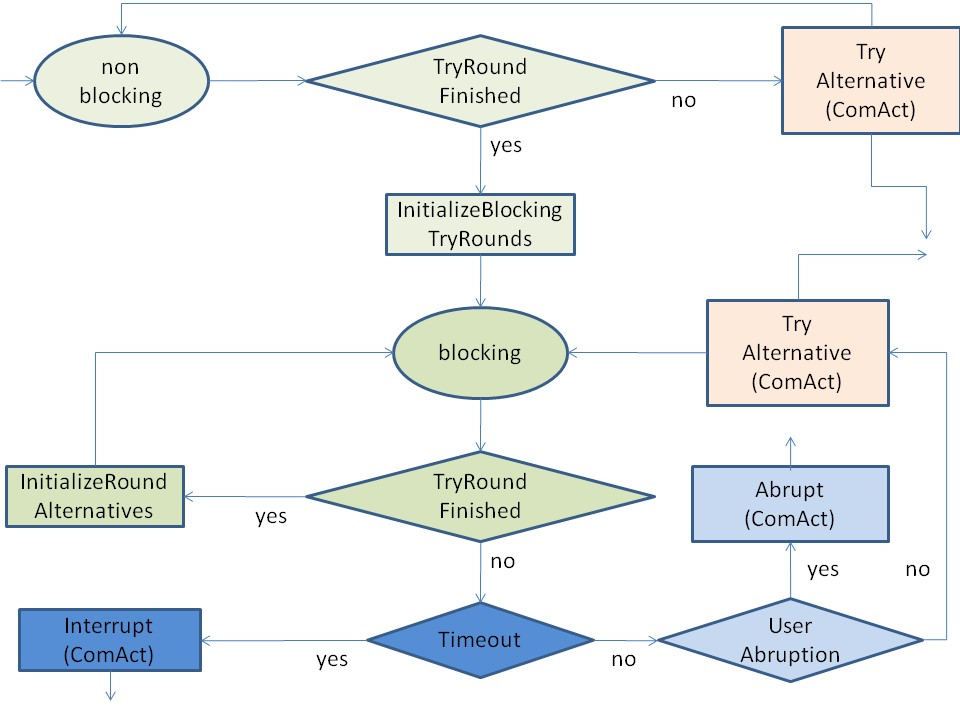
\includegraphics[width=0.8\linewidth]{20181026-Ontologie-Bilder/Grafiken-Ontologie/SUbjectExecution/ASM-Perform-Bild}
	\caption[Diagram of Alternative Send/Receive Round Interpretation]{Diagram of Alternative Send/Receive Round Interpretation}
	\label{fig:asm-perform-bild}
\end{figure}


\textbf{Interpretation of Auxiliary Macros}
\begin{figure}[ph]
	\centering
	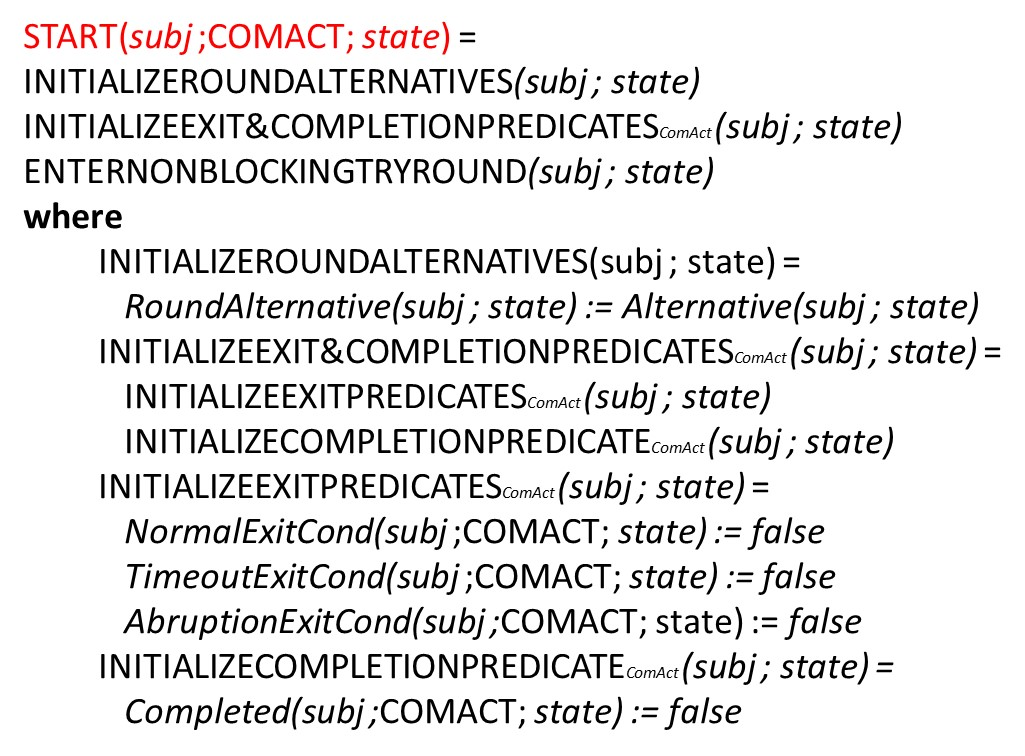
\includegraphics[width=0.8\linewidth]{20181026-Ontologie-Bilder/Grafiken-Ontologie/SUbjectExecution/ASM-Start}
	\caption[Start function]{Start function}
	\label{fig:asm-start}
\end{figure}

\begin{figure}
	\centering
	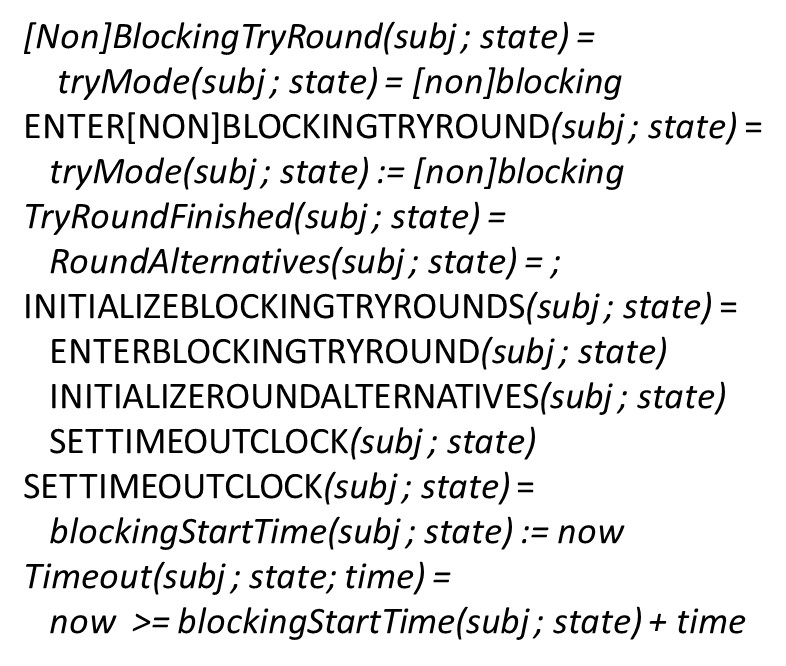
\includegraphics[width=0.8\linewidth]{20181026-Ontologie-Bilder/Grafiken-Ontologie/SUbjectExecution/ASM-Try-Run}
	\caption[Try non/blocking Round]{Try non/blocking Round}
	\label{fig:asm-try-run}
\end{figure}
%
\begin{figure}[ph]
	\centering
	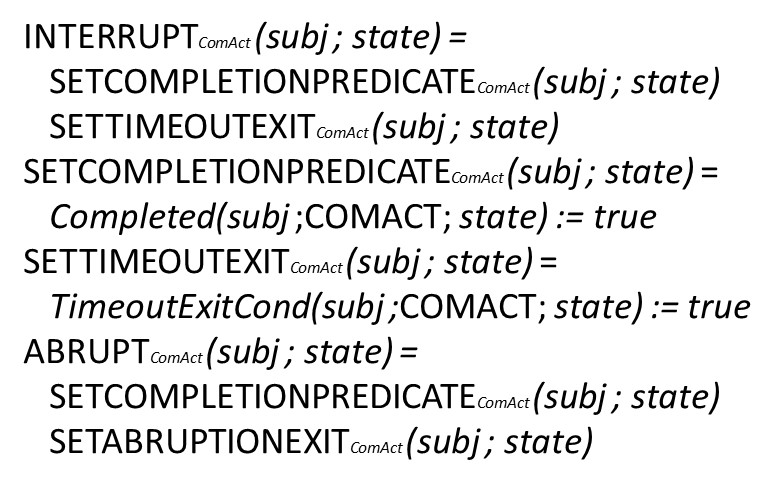
\includegraphics[width=0.8\linewidth]{20181026-Ontologie-Bilder/Grafiken-Ontologie/SUbjectExecution/ASM-Interrupt}
	\caption[Interupt Handling]{Interupt Handling}
	\label{fig:asm-interrupt}
\end{figure}

\newpage
\section{MsgElaboration Interpretation for Multi Send/Receive}

\begin{figure}[ph]
	\centering
	%\includegraphics[width=0.8\linewidth]{20181026-Ontologie-Bilder/Grafiken-Ontologie/SUbjectExecution/ASM-Message-Elaboration}
	\caption[Interpretation for Multi Send/Receive]{Interpretation for Multi Send/Receive}
	\label{fig:asm-Message-Elaboration}
\end{figure}



%
%
\section{Multi Send/Receive Round Interpretation}

\begin{figure}[ph]
	\centering
	%\includegraphics[width=0.8\linewidth]{20181026-Ontologie-Bilder/Grafiken-Ontologie/SUbjectExecution/ASM-Multi-Send}
	\caption{State Diagram Multi Send}
	\label{fig:ASM-Multi-Send}
\end{figure}

\begin{figure}[ph]
	\centering
	%\includegraphics[width=0.8\linewidth]{20181026-Ontologie-Bilder/Grafiken-Ontologie/SUbjectExecution/ASM-Multi-Receive}
	\caption{State Diagram Multi Receive}
	\label{fig:ASM-Multi-Receive}
\end{figure}

\begin{figure}[ph]
	\centering
	%\includegraphics[width=0.8\linewidth]{20181026-Ontologie-Bilder/Grafiken-Ontologie/SUbjectExecution/ASM-Multi-Send-Receive}
	\caption{ASM Interpreter for Multi Send/Receive}
	\label{fig:ASM-Multi-Send-Receive}
\end{figure}



\newpage




%%%%%%%%%%%%%%%%%%%%%%%%%%%%%%%%%%%%%%%%%%%%%%%%%%%%%%%%%%%%%%%
\section{Actual Send Interpretation}

\begin{figure}[ph]
	\centering
	%\includegraphics[width=0.8\linewidth]{20181026-Ontologie-Bilder/Grafiken-Ontologie/SUbjectExecution/ASM-Asynch-send}
	\caption[Interpretation for asynchronous send]{Interpretation for asynchronous send}
	\label{fig:asm-async-send}
\end{figure}

\begin{figure}
	\centering
	%\includegraphics[width=0.8\linewidth]{20181026-Ontologie-Bilder/Grafiken-Ontologie/SUbjectExecution/ASM-synch-send}
	\caption[Interpretation for synchronous send]{Interpretation for synchronous send}
	\label{fig:asm-sync-send}
\end{figure}

\newpage
%%%%%%%%%%%%%%%%%%%%%%%%%%%%%%%%%%%%%%%%%%%%%%%%%%%%%%%%%%%%%%%
\section{Actual Receive Interpreation}


\begin{figure}[ph]
	\centering
	%\includegraphics[width=0.8\linewidth]{20181026-Ontologie-Bilder/Grafiken-Ontologie/SUbjectExecution/ASM-Async-receive}
	\caption[Interpretation for asynchronous send]{Interpretation for asynchronous receive}
	\label{fig:asm-async-receive}
\end{figure}

\begin{figure}
	\centering
	%\includegraphics[width=0.8\linewidth]{20181026-Ontologie-Bilder/Grafiken-Ontologie/SUbjectExecution/ASM-sync-receive}
	\caption[Interpretation for asynchronous send]{Interpretation for synchronous receive}
	\label{fig:asm-sync-receive}
\end{figure}

%
%
%%%%%%%%%%%%%%%%%%%%%%%%%%%%%%%%%%%%%%%%%%%%%%%%%%%%%%%%%%%%%%%
\newpage
\section{Alternative Action Interpretation}
%
\begin{figure}[ph]
	\centering
	%\includegraphics[width=0.8\linewidth]{20181026-Ontologie-Bilder/Grafiken-Ontologie/SUbjectExecution/ASM-alternative-action}
	\caption[Alternative Actions]{Alternative Actions}
	\label{fig:asm-alternative-action}
\end{figure}
%
\begin{figure}
	\centering
	%\includegraphics[width=0.8\linewidth]{20181026-Ontologie-Bilder/Grafiken-Ontologie/SUbjectExecution/ASM-altaction-start-perform}
	\caption[Start and Perform Alternative Actions]{Start and Perform Alternative Actions}
	\label{fig:asm-alt-actions-perform}
\end{figure}
%
\begin{figure}
	\centering
	%\includegraphics[width=0.8\linewidth]{20181026-Ontologie-Bilder/Grafiken-Ontologie/SUbjectExecution/ASM-altaction-auxilary}
	\caption[Auxiliary Wait/Exit Rule Interpretation]{Auxiliary Wait/Exit Rule Interpretation}
	\label{fig:asm-alternative-action}
\end{figure}
%
%
%
\newpage
\section{Interrupt Behavior}
\begin{figure}[ph]
	\centering
	%\includegraphics[width=0.8\linewidth]{20181026-Ontologie-Bilder/Grafiken-Ontologie/SUbjectExecution/ASM-Interrupt-Behaviour}
	\caption[Interrupt-Behaviour]{Interrupt Behaviour (Guard)}
	\label{fig:ASM-Interrupt-Behaviour}
\end{figure}
